\documentclass[12pt,aspectratio=43]{beamer}

\usepackage{amssymb,amsmath,mathtext}
\usepackage{indentfirst,amsfonts}
\usepackage{makecell,multirow,longtable}

\usepackage[english,russian]{babel}
\usepackage[T2A]{fontenc}
\usepackage[utf8]{inputenc}


\graphicspath{{img/}}

%\usepackage{euscript}

\setbeamertemplate{navigation symbols}{}

%\usetheme{Warsaw}Boadilla,Pittsburgh,
%boxes,default,EastLansing
%Luebeck,Madrid,Szeged
\usetheme{EastLansing} 
%AnnArbor,Boadilla,EastLansing

%albatross,
%beaver, beetle, crane, dolphin, dove, fly, lily, orchid, rose, seagull, seahorse, sidebartab,
%structure, whale и wolverine
\usecolortheme{dove}%dove


\usepackage[square,numbers]{natbib}
\setcitestyle{authoryear, open={[},close={]}}
% These packages are all incorporated in the memoir class to one degree or another...
%\usepackage{tempora}
\let\bibhang\relax
\let\citename\relax
\let\bibfont\relax
\let\Citeauthor\relax
\let\bibsection\relax
\expandafter\let\csname ver@natbib.sty\endcsname\relax
\usepackage[backend=bibtex,style=numeric]{biblatex}  %backend=biber is 'better'  

\addbibresource{kursach.bib}

%%% ToC (table of contents) APPEARANCE
%\usepackage[nottoc,notlof,notlot]{tocbibind} % Put the bibliography in the ToC
%\usepackage[titles,subfigure]{tocloft} % Alter the style of the Table of Contents
%\renewcommand{\cftsecfont}{\rmfamily\mdseries\upshape}
%\renewcommand{\cftsecpagefont}{\rmfamily\mdseries\upshape} % No bold!
%\linespread{1.5}


\beamersetuncovermixins{\opaqueness<1>{30}}{\opaqueness<2->{25}}

\setbeamerfont{frametitle}{series=\bfseries}
\setbeamerfont{block title}{series=\bfseries}

\makeatletter
\defbeamertemplate*{footline}{my theme}{
	\leavevmode%
	\hbox{%
	\begin{beamercolorbox}[wd=.205\paperwidth,ht=2.25ex,dp=1ex,center]{author in head/foot}%
		\usebeamerfont{author in head/foot}%
		\insertshortauthor~\beamer@ifempty{}{}{(\insertshortinstitute)}
	\end{beamercolorbox}%
	\begin{beamercolorbox}[wd=.605\paperwidth,ht=2.25ex,dp=1ex,center]{title in head/foot}%
		\usebeamerfont{title in head/foot}\inserttitle
	\end{beamercolorbox}%
	\begin{beamercolorbox}[wd=.19\paperwidth,ht=2.25ex,dp=1ex,center]{date in head/foot}%
		%\usebeamerfont{date in head/foot}\insertshortdate{}\hspace*{.3em}	
\insertframenumber{}/\inserttotalframenumber\hspace*{1ex}
	\end{beamercolorbox}}%
}
\makeatother



\begin{document}
\title{Сравнение тригонометрических параллаксов звезд TGAS и Hipparcos}
\subtitle[Диплом]{Дипломная работа}
%\subtitle[short subtitle]{long subtitle}
\author[А.С.\,Патшин]{Патшин Антон Сергеевич\\{\footnotesize\textcolor{gray}{научный руководитель: доцент А.С.\,Цветков}}}
\date{} 


%\title[short title]{long title}
%\subtitle[short subtitle]{long subtitle}
%\author[short name]{long name}
%\date[short date]{long date}

\institute[СПбГУ]{Санкт-Петербургский государственный университет}


\maketitle

\section{Введение}
\subsection{Общие сведения о Hips}
\label{sub:smthhip}

%\begin{frame}\frametitle{Считалка} 

%  \begin{itemize}
%  \item гомоморфный образ группы
%  \item изопорфен фактор группе
%  \item {\Large \textcolor{blue}{до победы коммунизма!}}
%  \item по ядру гомоморфизма!
%  \end{itemize}
%\begin{equation}
%    Русский_{низ}^{вверх} = \frac{всё}{работает^2\dots} = E = m c^2
%\end{equation}

%\begin{block}{Introduction to {\LaTeX}}
%"Beamer is a {\LaTeX}class for creating presentations %that
%are held using a projector..."
%\end{block}
%\end{frame}


%\subsection{Общие сведения о Gaia}
%\label{sub:smthgaia}
%\begin{frame}\frametitle{Название кадра}

% 	\begin{columns}
% 		\column{0.5\textwidth}
% 			Тут табличка о hipparcos
 			 
% 		\column{0.5\textwidth}
% 			Тут табличка о Gaia (tgas)
 			 
% 	\end{columns}
%\end{frame}


\subsection{Постановка задачи и Актуальность}

\label{sub:smthgaia}
\begin{frame}\frametitle{Введение}
\begin{block}{Постановка задачи}
\begin{itemize}
  \item Высокая формальная точность Hipparcos и TGAS
  \item Указание на систематические ошибки параллаксов Hipparcos (в том числе, аппарат Hubble, 2007)
  \item \textbf{Впервые} появилась возможность сравнить параллаксы (ранее только координаты и с.д.) – стандартная астрометрическая задача
  \end{itemize}
\end{block}
\begin{block}{Актуальность}
\begin{itemize}
  \item[] Миссия Gaia (TGAS) – в процессе.
\end{itemize}
\end{block}
\end{frame}

\subsection{Каталоги}
\begin{frame}%\frametitle{}
\begin{block}{Каталог Hipparcos}
\begin{itemize}
  \item Содержит 118 324 объекста
  \end{itemize}
\end{block}  

\begin{block}{Подкаталог TGAS}
\begin{itemize}
  \item Tycho-2 (1 963 415)
  \item Hipparcos (93 635)
  \end{itemize}
\end{block}  
\begin{block}{Объединённый каталог}
\begin{itemize}
  \item Пересечение Hip и TGAS
  \item 90 283 объекта
  \end{itemize}
\end{block}  
\end{frame}	


\begin{frame}%\frametitle{Введение}
%\frametitle{Визуализация распределения}
\begin{figure}[h!]
\center{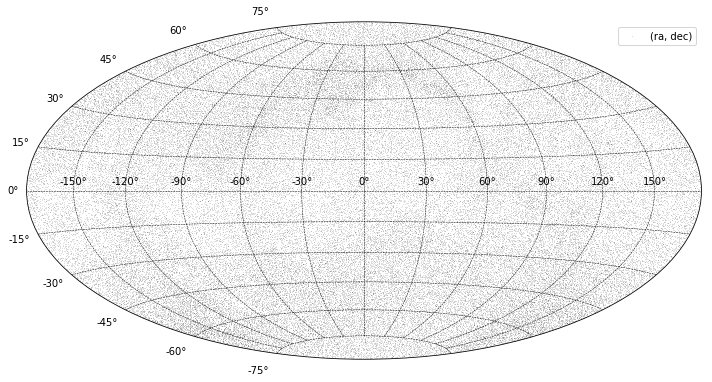
\includegraphics[width=.9\linewidth]{hiptgasra}}\\{Распределение звезд из объединённого каталога в экваториальной СК}
%\label{img:hiptgasra}
\end{figure}
\end{frame}	


\begin{frame}[<alignment>]
\begin{figure}[H]
\begin{minipage}[h]{0.47\linewidth}
\center{\includegraphics[width=1\linewidth]{hist_dif7}\\{Гистограмма разности параллаксов общего каталога}} 
\end{minipage}
\hfill
\begin{minipage}[h]{0.47\linewidth}
\center{\includegraphics[width=1\linewidth]{hist_dif7abs}\\{Гистограмма модуля разности параллаксов общего каталога}} 
\end{minipage}
%\caption{инстуременты разработки}
%\label{ris:experimentalcorrelationsignals}
\end{figure}
\end{frame}

%\begin{frame}[<alignment>]
%\frametitle{}
%\begin{figure}[h!]
%\center{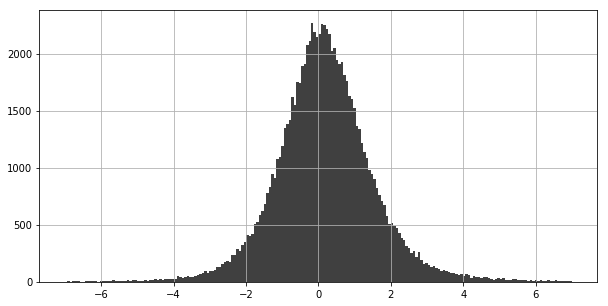
\includegraphics[width=.87\linewidth]{hist_par_deff}}
%\caption{Гистограмма разности параллаксов общего каталога.}
%\label{img:hist_par_deff}
%\end{figure}
%\end{frame}

\section{Случайные выбросы}\label{sub:smthrs}

\begin{frame}
\frametitle{Случайные выбросы}
\begin{block}{}
\begin{itemize}
  \item[  ] Большие выбросы : звезды, для которых модуль разности превосходит 15 mas (Хаммер-Айтофа, в описании Hipparcos).
\end{itemize}
\end{block}

\begin{figure}[h!]
\center{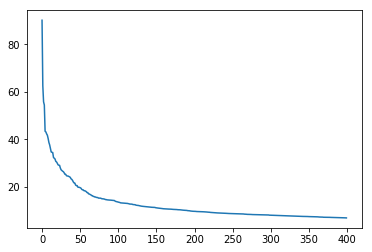
\includegraphics[width=.57\linewidth]{abs_paralax}}
\caption{График убывания модуля разностей параллаксов.}
%\label{img:abs_paralax}
\end{figure}

\end{frame}

\subsection{Проекция Хаммер-Айтофа}\label{sub:hammer}

\begin{frame}[<alignment>]
\frametitle{Проекция Хаммер-Айтофа}
\begin{figure}[h!]
\center{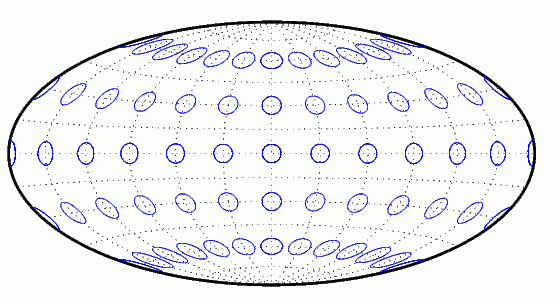
\includegraphics[width=1.\linewidth]{hammtiss}}
\label{img:hammtiss}
\end{figure}
\end{frame}	

\subsection{Визуализация распределения}\label{sub:smthrs}

\begin{frame}[<alignment>]
%\frametitle{Случайные выбросы}

\begin{figure}[h!]
\center{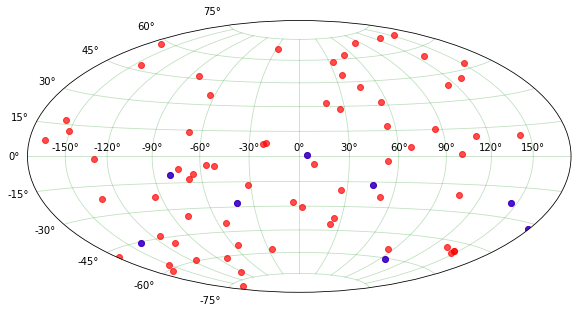
\includegraphics[width=1.\linewidth]{75maxradec}}
\caption{Распределение рекордсменов в экваториальной СК  Красные - положительные, синие - отрицательные.}
%\label{img:75maxradec}
\end{figure}
\end{frame}




\subsection{Построение и предварительный анализ}\label{errvid}

\begin{frame}[squeeze, shrink=5]
\frametitle{Построение и предварительный анализ}
\begin{table}[h!]
%\centering
\caption{Общие статистики по объединённому каталогу}
\label{tabular:tgas_st}
\begin{tabular}{c|r|r|r|r|r|r|r}
%\rowcolor{Gray} 
\hline 	
&$\pi_{tgas}$&$\pi_{hip}$&$\pi_{dif}$&$\pi_{dif_{abs}}$&$\delta_{\pi_{tgas}}$&$\delta_{\pi_{hip}}$&$n_{obs}$\\
\hline
\hline 	
count&90283&90283&90283&90283&90283&90283&90283\\
\hline 
mean&6.812&7.02&0.21&1.07&0.33&1.05&117.48\\
std&8.564&8.64&1.71&1.35&0.13&0.82&42.86\\
min&0.002&0.01&-42.35&5.4e-07&0.20&0.09&20\\
25\%&2.506&2.67&-0.61&0.35&0.24&0.68&86\\
50\%&4.369&4.66&0.14&0.77&0.28&0.91&113\\
75\%&7.984&8.33&0.93&1.40&0.35&1.21&140\\
max&295.8&298.0&90.05&90.05&0.99&47.48&388\\
\end{tabular}
\end{table}

\end{frame}	



\section{Систематические различия}\label{sistem}

\subsection{Healpix}\label{sub:smthhealpix}
\begin{frame}[<alignment>]
\frametitle{HEALPix}

\begin{figure}[h!]
\center{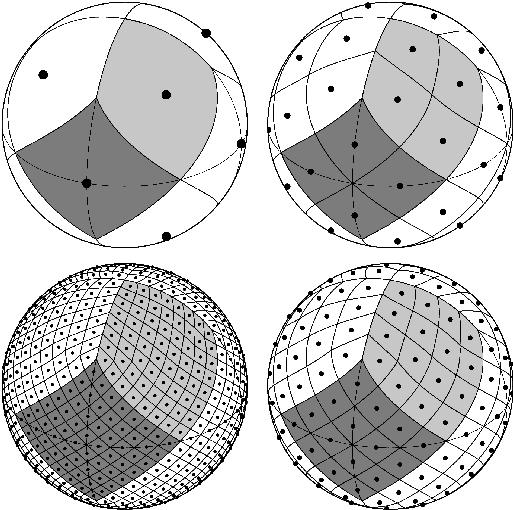
\includegraphics[width=0.6\linewidth]{healpix}}
\label{img:healpix}
\end{figure}

\end{frame}	

\begin{frame}[<alignment>]
\begin{figure}[h!]
\center{\includegraphics[width=1.\linewidth]{healpix_1200}}
\label{img:healpix}
\end{figure}
.\end{frame}	

\subsection{Распределение}\label{sub:smthhealpix}

\begin{frame}[<alignment>]
\frametitle{Распределение}
\begin{figure}[h!]
\center{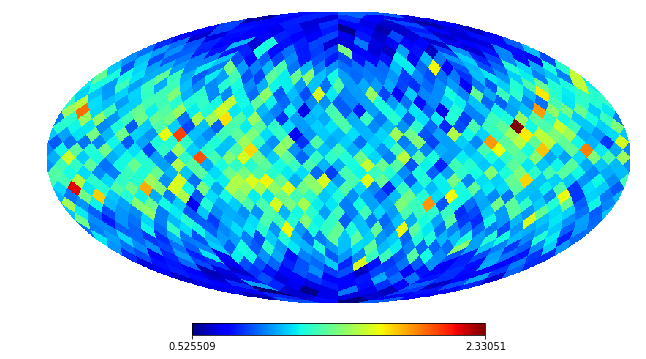
\includegraphics[width=0.7\linewidth]{sf_lo}}\\{Распределение модуля разности параллаксов в эклиптической СК}
%\caption{Распределение модуля параллаксов в эклиптической СК}
\label{img:sf_lo}
\end{figure}

\end{frame}	

\subsection{Сферические функции}\label{sistem}  
\begin{frame}[<alignment>]
%\begin{block}{Сфрические функции} %\frametitle{Сферические функци}
\begin{equation}\label{f:sf_prll} 
\Delta_{plx} (l,b) = \sum_{nkp}\beta_{nkp}K_{nkp}(l,b),
\end{equation}

\begin{equation}\label{f:sf_k}
K_{nkp}(l,b) = R_{nk} \left\{ \begin{array}{ll}
P_{n,0}(b), & \textrm{$k=0, p=1$,}\\
P_{n,k}(b)\sin{kl}, & \textrm{$k\neq0, p=0$,}\\
P_{n,k}(b)\cos{kl}, & \textrm{$k\neq0, p=1$,}
\end{array} \right.
\end{equation}

\begin{equation}\label{f:sf_R}
R_{nk} = \sqrt[]{\frac{2n+1}{4\pi}} \left\{ \begin{array}{cc}
\sqrt[]{\frac{2(n-k)!}{(n+k)!}}, & \textrm{$k>0$,}\\
1, & \textrm{$k=0$,}
\end{array} \right.
\end{equation}

$P_{nk}(b)$ - полиномы Лежандра (при $k = 0$) и присоединенные функции Лежандра (при $k > 0$)
\begin{equation}\label{f:sf_pl}
\begin{array}{rll}
P_{nk}(b)&=\sin{b\frac{2n-1}{n-k}}P_{n-1,k}(b)-\frac{n+k-1}{n-k}P_{n-2,k}(b),{}^{k=0,1,..}_{n=k+1,k+2,..}\\
P_{kk}(b)&=\frac{(2k)!}{2^{k}k!}{\cos{b}}^{k},\\
P_{k+1,k}(b)&=\frac{(2k+2)!}{2^{k+1}(k+1)!}{\cos{b}}^{k}\sin{b}.
\end{array}
\end{equation}
\begin{equation}\label{f:sf_j}
j = n^2 + 2k + p -1.
\end{equation}
%\end{block}
\end{frame}	


\begin{frame}
\frametitle{Сферически функции от 1 до 16}
\begin{figure}[H]
\begin{minipage}[h]{0.23\linewidth}
\center{\includegraphics[width=1\linewidth]{moll_nside_1}} 
\end{minipage}
\hfill
\begin{minipage}[h]{0.23\linewidth}
\center{\includegraphics[width=1\linewidth]{moll_nside_2}} 
\end{minipage}
\hfill
\begin{minipage}[h]{0.23\linewidth}
\center{\includegraphics[width=1\linewidth]{moll_nside_3}} 
\end{minipage}
\hfill
\begin{minipage}[h]{0.23\linewidth}
\center{\includegraphics[width=1\linewidth]{moll_nside_4}} 
\end{minipage}
\vfill

\begin{minipage}[h]{0.23\linewidth}
\center{\includegraphics[width=1\linewidth]{moll_nside_5}} 
\end{minipage}
\hfill
\begin{minipage}[h]{0.23\linewidth}
\center{\includegraphics[width=1\linewidth]{moll_nside_6}} 
\end{minipage}
\hfill
\begin{minipage}[h]{0.23\linewidth}
\center{\includegraphics[width=1\linewidth]{moll_nside_7}} 
\end{minipage}
\hfill
\begin{minipage}[h]{0.23\linewidth}
\center{\includegraphics[width=1\linewidth]{moll_nside_8}} 
\end{minipage}
\vfill

\begin{minipage}[h]{0.23\linewidth}
\center{\includegraphics[width=1\linewidth]{moll_nside_9}} 
\end{minipage}
\hfill
\begin{minipage}[h]{0.23\linewidth}
\center{\includegraphics[width=1\linewidth]{moll_nside_10}} 
\end{minipage}
\hfill
\begin{minipage}[h]{0.23\linewidth}
\center{\includegraphics[width=1\linewidth]{moll_nside_11}} 
\end{minipage}
\hfill
\begin{minipage}[h]{0.23\linewidth}
\center{\includegraphics[width=1\linewidth]{moll_nside_12}} 
\end{minipage}
\vfill

\begin{minipage}[h]{0.23\linewidth}
\center{\includegraphics[width=1\linewidth]{moll_nside_13}} 
\end{minipage}
\hfill
\begin{minipage}[h]{0.23\linewidth}
\center{\includegraphics[width=1\linewidth]{moll_nside_14}} 
\end{minipage}
\hfill
\begin{minipage}[h]{0.23\linewidth}
\center{\includegraphics[width=1\linewidth]{moll_nside_15}} 
\end{minipage}
\hfill
\begin{minipage}[h]{0.23\linewidth}
\center{\includegraphics[width=1\linewidth]{moll_nside_16}} 
\end{minipage}

%\caption{инстуременты разработки}
%\label{ris:experimentalcorrelationsignals}
\end{figure}
\end{frame}


\subsection{Сферические гармоники}\label{sistem}  
\begin{frame}[<alignment>]
\frametitle{Сферические гармоники}

\begin{figure}[h!]
\center{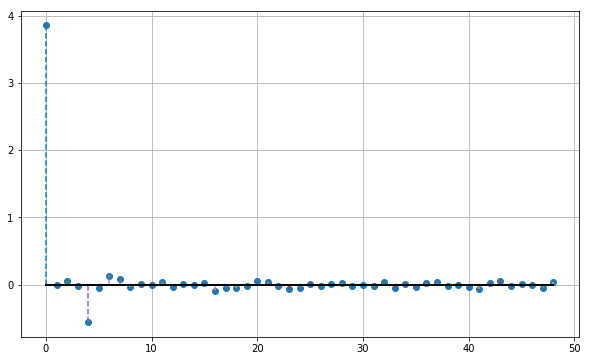
\includegraphics[width=1\linewidth]{sf_j}}
\caption{Гармоники эклиптической СК}
\label{img:sf_j}
\end{figure}
\end{frame}	

\begin{frame}[<alignment>]
\frametitle{Сферические гармоники}
\begin{table}[h]
\centering
\caption{Значимые гармоники в эклиптической СК с мат. ожиданием и стандартным отклонением}
\label{tabular:sf_04}
\begin{tabular}{|c|c|c|c|}
\hline 	
$j$ &$\beta_{j,(lon,lat)}$ & $\mu(\beta_{lon,lat})$ & $\sigma(\beta_{lon,lat})$\\
\hline 	
0 &3.8569 &0.0663 &0.5541\\
4 &-0.5543 &0.0663 &0.5541\\
\hline 	
\end{tabular}
\end{table}
\end{frame}	

\begin{frame}
\frametitle{Сферические гармоники}
\begin{figure}[h!]
\center{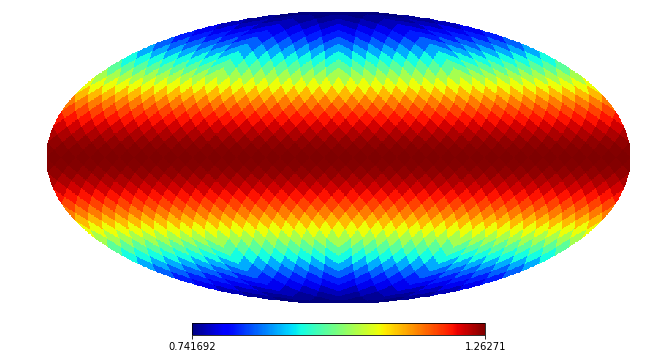
\includegraphics[width=0.97\linewidth]{sfff}}
\caption{Значимые (0.4) гармоники в эклиптической СК}
\label{img:sfff}
\end{figure}
\end{frame}	

\begin{frame}[<alignment>]
\frametitle{Сферические гармоники}
\begin{figure}[h!]
\center{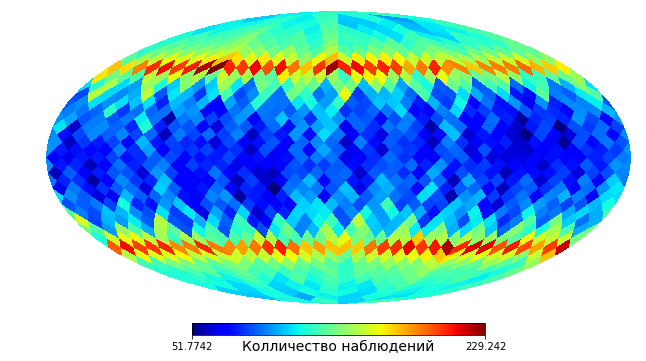
\includegraphics[width=0.97\linewidth]{nobs}}\\{Распределение числа наблюдения звезд в эклиптической СК}
%\caption{}
\label{img:nobs}
\end{figure}
\end{frame}	


\section{Заключение}\label{conclusion}
\begin{frame}
\frametitle{Заключение}

\begin{block}{}
\begin{itemize}
  \item Звезды по HIP ближе на $6\%$.
  \item Cсистематически параллаксы сильно не различаются -- TGAS использовались первые эпохи из Hipparcos и Tycho-2 -- видимо данные с ними коррелированны.
\end{itemize}
\end{block}
\end{frame}	

\begin{frame}
\frametitle{Заключение}
 Результаты Hipparcos принимались за абсолютную истину, хотя были факты, указывающие на резкое противоречие с данными наземных наблюдений. Выявление сист. ошибок – только сравнение с другими каталогами, полученными незваисимо. Кроме того выявлены «рекордсмены» - звезды с явно разными параллаксами.
\end{frame}


\begin{frame}
\frametitle{Спасибо за внимание!}
\begin{figure}[h!]
\center{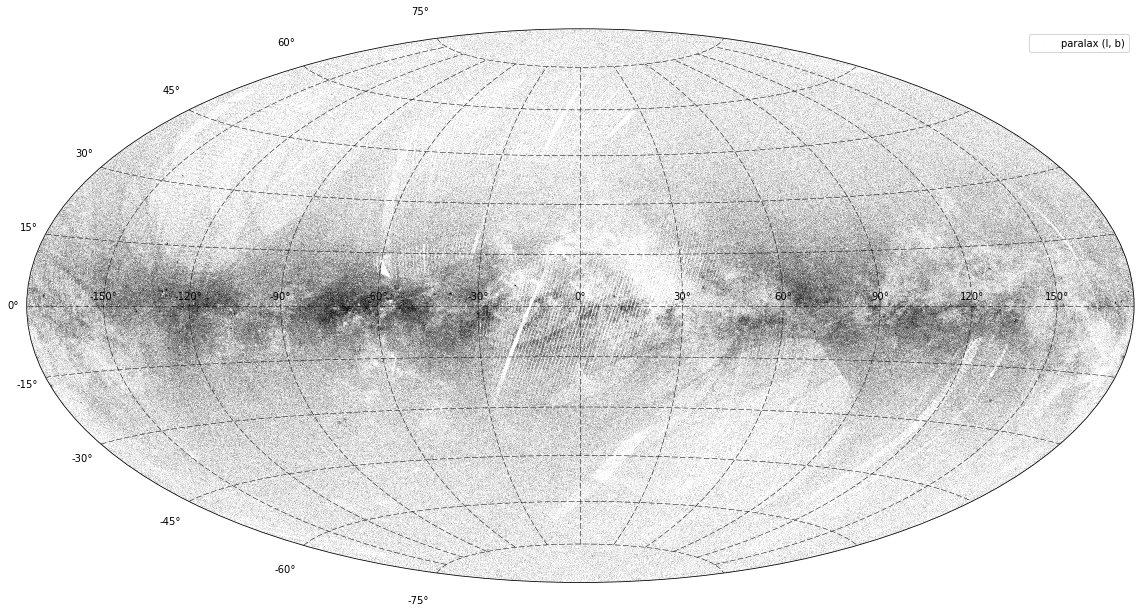
\includegraphics[width=1\linewidth]{alllv}}
%\caption{Гармоники эклиптической СК}
\label{img:alllv}
\end{figure}
\end{frame}

%\setcounter{framenumber}{0} %or \setcounter{framenumber}{1}

%\setcounter{framenumber}{\value{finalframe}}
\appendix
\newcounter{finalframe}
\setcounter{finalframe}{\value{framenumber}}

\begin{frame}
\section{Список использованной литературы}\label{conclusionlit}
%\bibliographystyle{unsrt}
%\bibliography{kursach.bib}
\printbibliography[type=online,title={Сайты}]
\printbibliography[type=book,title={Статьи:}]
\end{frame}



\begin{frame}

\frametitle{Инструменты которыми, пользовались в исследования}
\begin{figure}[H]
\begin{minipage}[h]{0.12\linewidth}
\center{\includegraphics[width=0.85\linewidth]{c_logo}} 
\end{minipage}
\hfill
\begin{minipage}[h]{0.12\linewidth}
\center{\includegraphics[width=.53\linewidth]{ISO_C++_Logo}} 
\end{minipage}
\hfill
\begin{minipage}[h]{0.3\linewidth}
\center{\includegraphics[width=.8\linewidth]{fortran}} 
\end{minipage}
\hfill
\begin{minipage}[h]{0.3\linewidth}
\center{\includegraphics[width=.5\linewidth]{python}} 
\end{minipage}

\vfill
\begin{minipage}[h]{0.31\linewidth}
\center{\includegraphics[width=0.85\linewidth]{IPy_header}} 
\end{minipage}
\hfill
\begin{minipage}[h]{0.31\linewidth}
\center{\includegraphics[width=.5\linewidth]{jupyter_logo}} 
\end{minipage}
\hfill
\begin{minipage}[h]{0.31\linewidth}
\center{\includegraphics[width=.5\linewidth]{Anaconda_Logo}} 
\end{minipage}

\vfill
\begin{minipage}[h]{0.31\linewidth}
\center{\includegraphics[width=0.6\linewidth]{numpy_logo}} 
\end{minipage}
\hfill
\begin{minipage}[h]{0.31\linewidth}
\center{\includegraphics[width=.995\linewidth]{pandas_logo}} 
\end{minipage}
\hfill
\begin{minipage}[h]{0.31\linewidth}
\center{\includegraphics[width=.5\linewidth]{scipy}} 
\end{minipage}
\vfill

\begin{minipage}[h]{0.47\linewidth}
\center{\includegraphics[width=.35\linewidth]{220px-LaTeX_logo}} 
\end{minipage}
\hfill
\begin{minipage}[h]{0.47\linewidth}
\center{\includegraphics[width=.65\linewidth]{nplotlib_logos2}} 
\end{minipage}
%\caption{инстуременты разработки}
%\label{ris:experimentalcorrelationsignals}
\end{figure}
\end{frame}


\begin{frame}[<alignment>]
%\frametitle{Визуализация распределения}
\begin{figure}[h!]
\center{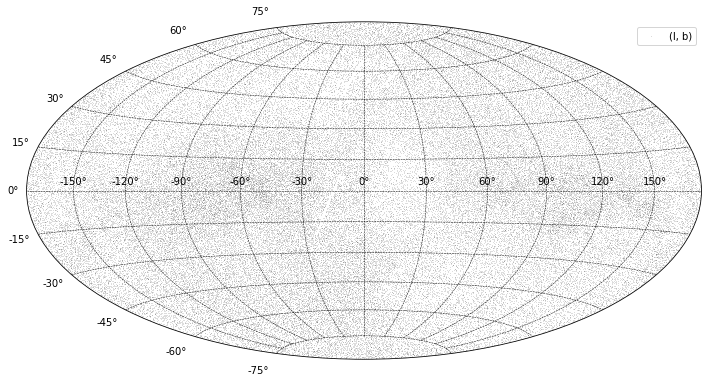
\includegraphics[width=1\linewidth]{hiptgasl}}
\caption{Распределение в галлактической СК}
\label{img:hiptgasl}
\end{figure}
\end{frame}	

\begin{frame}[<alignment>]
%\frametitle{Визуализация распределения}
\begin{figure}[h!]
\center{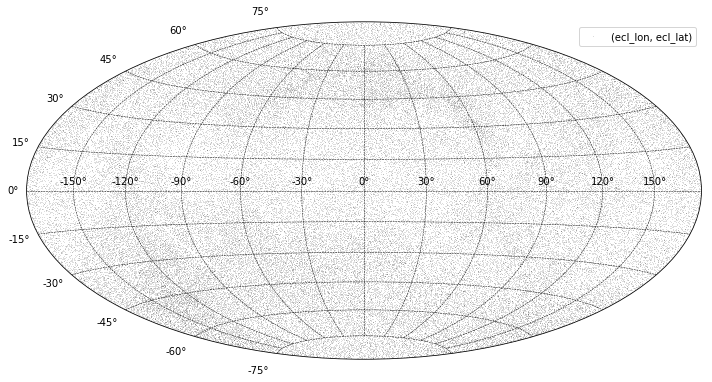
\includegraphics[width=1.\linewidth]{hiptgaslo}}
\caption{Распределение в эклиптической СК}
\label{img:hiptgaslo}
\end{figure}
\end{frame}	



\begin{frame}[<alignment>]
%\frametitle{Случайные выбросы}
\begin{figure}[h!]
\center{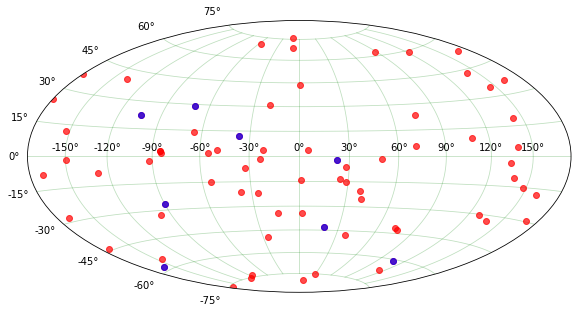
\includegraphics[width=1.\linewidth]{75maxlb}}
\caption{Распределение рекордсменов в галактической СК Красные - положительные, синие - отрицательные.}
\label{img:75maxlb}
\end{figure}
\end{frame}

\begin{frame}[<alignment>]
%\frametitle{Случайные выбросы}
\begin{figure}[h!]
\center{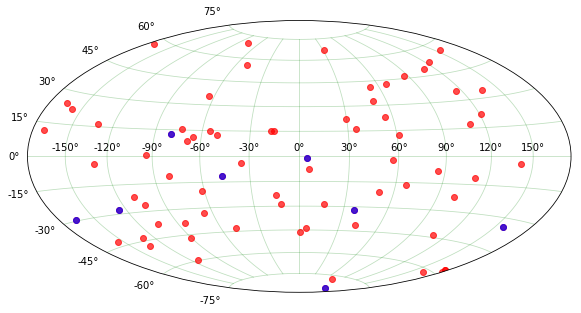
\includegraphics[width=1.\linewidth]{75maxlonlat}}
\caption{Распределение рекордсменов в эклиптической СК Красные - положительные, синие - отрицательные.}
\label{img:75maxlonlat}
\end{figure}
\end{frame}	

\begin{frame}[<alignment>]
\frametitle{Распределение разностей паралаксов}
\begin{figure}[h!]
\center{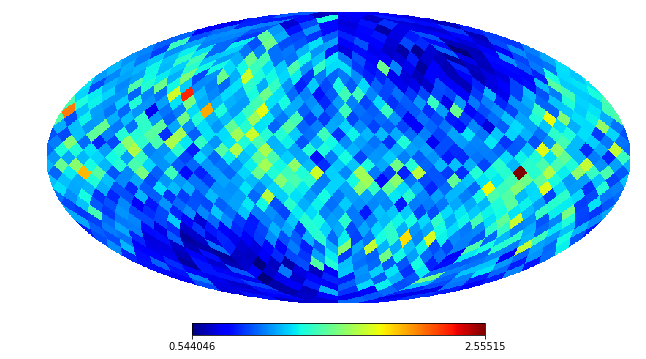
\includegraphics[width=0.7\linewidth]{sf_ra}}
\caption{Распределение модуля параллаксов в экваториальной СК }
\label{img:sf_ra}
\end{figure}
\end{frame}	

\begin{frame}[<alignment>]
\frametitle{Распределение разностей паралаксов}
\begin{figure}[h!]
\center{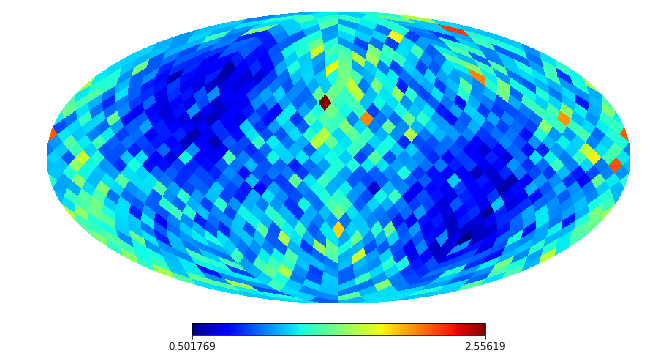
\includegraphics[width=0.7\linewidth]{sf_l}}
\caption{Распределение модуля параллаксов в галактической СК}
\label{img:sf_l}
\end{figure}

\end{frame}	

\setcounter{framenumber}{\value{finalframe}}
\end{document}